\chapter{اتّصال \lr{IMS} به شبکه\nf ی \lr{4G}}
\setlatintextfont{Times New Roman}
\label{imslte}
همانطور که در بخش\nf های قبل توضیح داده شد، \lr{IMS} می\nf تواند از طریق المان \lr{PGW} به معماری نسل چهارمِ ارتباطات متّصل شود. برای ارتباط پیاده\nf سازی \lr{clearwater} به \lr{VoLTE}(به\nf طوری که \lr{IMS} قادر به تعامل با المان\nf های شبکه\nf ی سلولی باشد)، نیاز به محصول تجاری \lr{Perimeta} می\nf باشد که توسّط شرکت \lr{Metaswitch} ارائه می\nf شود. همچنین، می\nf توان از \lr{PCRF} مورد استفاده توسّط اپراتورهای تلفن همراه نیز برای این کار استفاده کرد؛ امّا ممکن است که \lr{PCRF} مورد استفاده توسّط این اپراتورها، برخی قابلیت\nf ها مانند تضمین کیفیت سرویس را نداشته\nf باشد. با توجّه به مطالب فوق، تصمیم بر آن شد که \lr{clearwater}، به\nf عنوان یک ارائه\nf دهنده\nf ی سرویس \lr{VOIP}، به هسته\nf ی معماری نسل چهارم ارتباطات متّصل شود و قابلیّت برقراری تماس برای کاربران نسل چهارم از طریق سوئیچ بسته\nf ای فراهم شود.

\section{پیاده\nf سازی نسل چهارم ارتباطات}

\subsubsection{پیاده\nf سازی ها مختلف}

پیاده\nf سازی\nf های مختلفی برای معماری نسل چهارم ارائه شده\nf اند که یکی از مهم\nf ترین و کامل\nf ترین ِآن\nf ها، پیاده\nf سازی \lr{OpenAirInterface} است. \lr{OpenAirInterface}، یک پیاده\nf سازی متن\nf باز از نسل چهارم ارتباطات است که این معماری را در دو بخش \lr{eNB} و \lr{EPC} پیاده\nf سازی کرده است. \lr{srsLTE} نیز یک پیاده\nf سازی متن\nf باز است و در ابتدا فقط \lr{eNB} را پیاده\nf سازی کرده\nf بود ولی اخیراً، \lr{EPC} مخصوص به خود را نیز ارائه می\nf کند. پیاده\nf سازی\nf های دیگری نظیر \lr{Amarisoft} نیز وجود دارند. طبق بررسی\nf های انجام\nf شده، \lr{oai}\RTLfootnote{سرواژه\nf ی عبارت \lr{OpenAirInterface}. در این گزارش، منظور از \lr{oai}، پیاده\nf سازی نسل  چهارم ارتباطات توسّط \lr{OpenAirInterface} است. } و \lr{srs}\RTLfootnote{سرواژه\nf ی عبارت \lr{Software Radio System}. در این گزارش، منظور از \lr{srs}، پیاده\nf سازی نسل چهارم ارتباطات توسّط شرکت \lr{Software Radio System} است. }، بهترین پیاده\nf سازی\nf های موجودِ متن\nf باز از معماری نسل چهارم ارتباطات هستند. لذا در این پروژه، ابتدا عملکرد این دو پیاده\nf سازی مورد بررسی قرار گرفت و سپس گزینه\nf ی بهتر، برای اتّصال \lr{IMS} به \lr{4G} مورد استفاده قرار گرفت.

\subsubsection{مقایسه\nf ی  پیاده\nf سازی\nf های متن\nf باز \lr{oai} و \lr{srs}}


این امکان وجود دارد که  \lr{eNB} پیاده\nf سازی\nf شده توسّط \lr{srsLTE} را به \lr{EPC} پیاده\nf سازی\nf شده توسّط سایر شرکت\nf ها نظیر \lr{OpenAirInterface} و \lr{Amarisoft} متّصل کرد. در پژوهش \lr{Gringoli} و همکاران\cite{ltecomp}، مقایسه\nf ای برای بررسی عملکرد سیستم \lr{4G} در دو حالت مختلف انجام شده است. در هر دو حالت، از \lr{oai EPC} به عنوان هسته\nf ی شبکه استفاده شده است. در حالت اوّل، از \lr{oai eNB} و در حالت دوّم، از \lr{srs eNB} استفاده شده است. در این مقاله، با استفاده از سه دستگاه کاربر مختلف، نرخ ارسال(دریافت) داده\nf ها و همچنین میزان استفاده از \lr{CPU} توسّط سرورهای مورد استفاده، بررسی شده است. در مورد نرخ ارسال داده\nf ها، هر دو حالت تقریباً برابری می\nf کنند؛ امّا در استفاده از \lr{CPU}، حالت اوّل که از \lr{oai eNB} استفاده می\nf کند، بسیار عملکرد بهتری دارد و از توان \lr{CPU} کم\nf تری استفاده می\nf کند.

\subsubsection{پیاده\nf سازی \lr{oai} و \lr{srs}}

در انجام این پروژه، \lr{oai} و \lr{srs} پیاده\nf سازی شدند. در پیاده\nf سازی \lr{oai}\cite{weboai}، از گزارش پروژه\nf ی کارشناسی یک از دانشجویان\RTLfootnote{امیررضا بلوچی}  دانشکده برق و کامپیوتر دانشگاه صنعتی اصفهان تحت عنوان "پیاده\nf سازی نرم\nf افزاری شبکه\nf ی \lr{LTE}" استفاده شد. پس از پیاده\nf سازی \lr{oai}، تلفن همراه از طریق سیم\nf کارت پروگرام\nf شده، به هسته\nf ی شبکه متّصل شد و از طریق آن، به شبکه\nf ی محلّی دانشگاه و همچنین شبکه\nf ی اینترنت دسترسی پیدا کرد.

\lr{srs} با استفاده از مستندات موجود در \cite{websrs} پیاده\nf سازی شد\RTLfootnote{کل پروژه\nf ی \lr{srsLTE} پیاده\nf سازی شد. در این پیاده\nf سازی، هم در بخش \lr{eNB} و هم در بخش \lr{EPC}، از \lr{srs} استفاده شد. }. پس از پروگرام کردن سیم\nf کارت، متناسب با پیکربندی و اطّلاعات درون پایگاه داده\nf ی \lr{srs}، دستگاه کاربر با استفاده از سیم\nf کارت مذکور به \lr{srs eNB} متّصل شد. با مشاهده\nf ی بسته\nf های مبادله\nf شده بین \lr{srs EPC} و \lr{srs eNB}، مشخّص گردید که کاربر نمی\nf تواند به \lr{EPC} متّصل شود. با جستجو در تالار گفتمان \lr{srs} مشخّص شد که افراد دیگری نیز با همین مشکل روبه\nf رو شده\nf اند و راه\nf حلی یافت نشد. به احتمال زیاد، به دلیل این\nf که \lr{srs EPC} به\nf تازگی پیاده\nf سازی شده است، نیاز به رفع اشکال و عیب\nf یابی دارد. با توجّه به این مشکل و همچنین به دلیل عملکرد بهتره \lr{oai}، تصمیم گرفته\nf شد که این سیستم برای اتّصال به \lr{IMS} مورد استفاده قرار گیرد. 

\section{اتّصال \lr{IMS} به هسته\nf ی شبکه\nf ی \lr{4G}}

در پیاده\nf سازی \lr{oai}، نود \lr{eNB} از طریق کابل \lr{USB} به بورد \lr{USRP B210} متّصل می\nf شود و شبکه\nf ی دسترسی رادیویی را تشکیل می\nf دهند. نود \lr{EPC} نیز حاوی المان\nf های هسته\nf ی شبکه\nf ی سلولی است. این المان\nf ها عبارتند از:
\begin{itemize}
\item \lr{HSS}: مسئول نگهداری پروفایل دیتای مشترکین
\item \lr{MME}: مسئول مدیریت جابه\nf جایی
\item \lr{SPGW}: مسئول برقراری ارتباط با اینترنت و \lr{IMS}
\end{itemize}

معماری \lr{oai}، مطابق شکل \ref{oai} می\nf باشد.ابتدا بخش \lr{EPC} و \lr{eNB} بر روی دو رایانه\nf ی مجزّا نصب و پیکربندی شدند. پس از برقراری ارتباط بین \lr{EPC} و \lr{eNB} از طریق کابل اترنت، سیستم به\nf طور کامل راه\nf اندازی شد. سپس سیم\nf کارت\nf ها، متناسب با پیکربندی و اطّلاعات پایگاه داده\nf ی \lr{oai} پروگرام شدند. پس از قرار دادن سیم\nf کارت پروگرام\nf شده در دستگاه تلفن همراه، سیم\nf کارت با فرستادن سیگنال\nf های ارتباطی به بورد \lr{USRP B210}، ابتدا به \lr{oai eNB} متّصل شد. \lr{eNB} نیز اطّلاعات دریافت\nf شده از کاربر را به \lr{EPC} ارسال کرد و عمل ثبت\nf نام پایان یافت. پس از پایان ثبت\nf نام، کاربر با فعّال کردن دیتای تلفن همراه خود، می\nf تواند آدرس \lr{IP} به\nf دست آورد و  از طریق \lr{SPGW}، به اینترنت متّصل شود.

\begin{figure}[H]
\centering
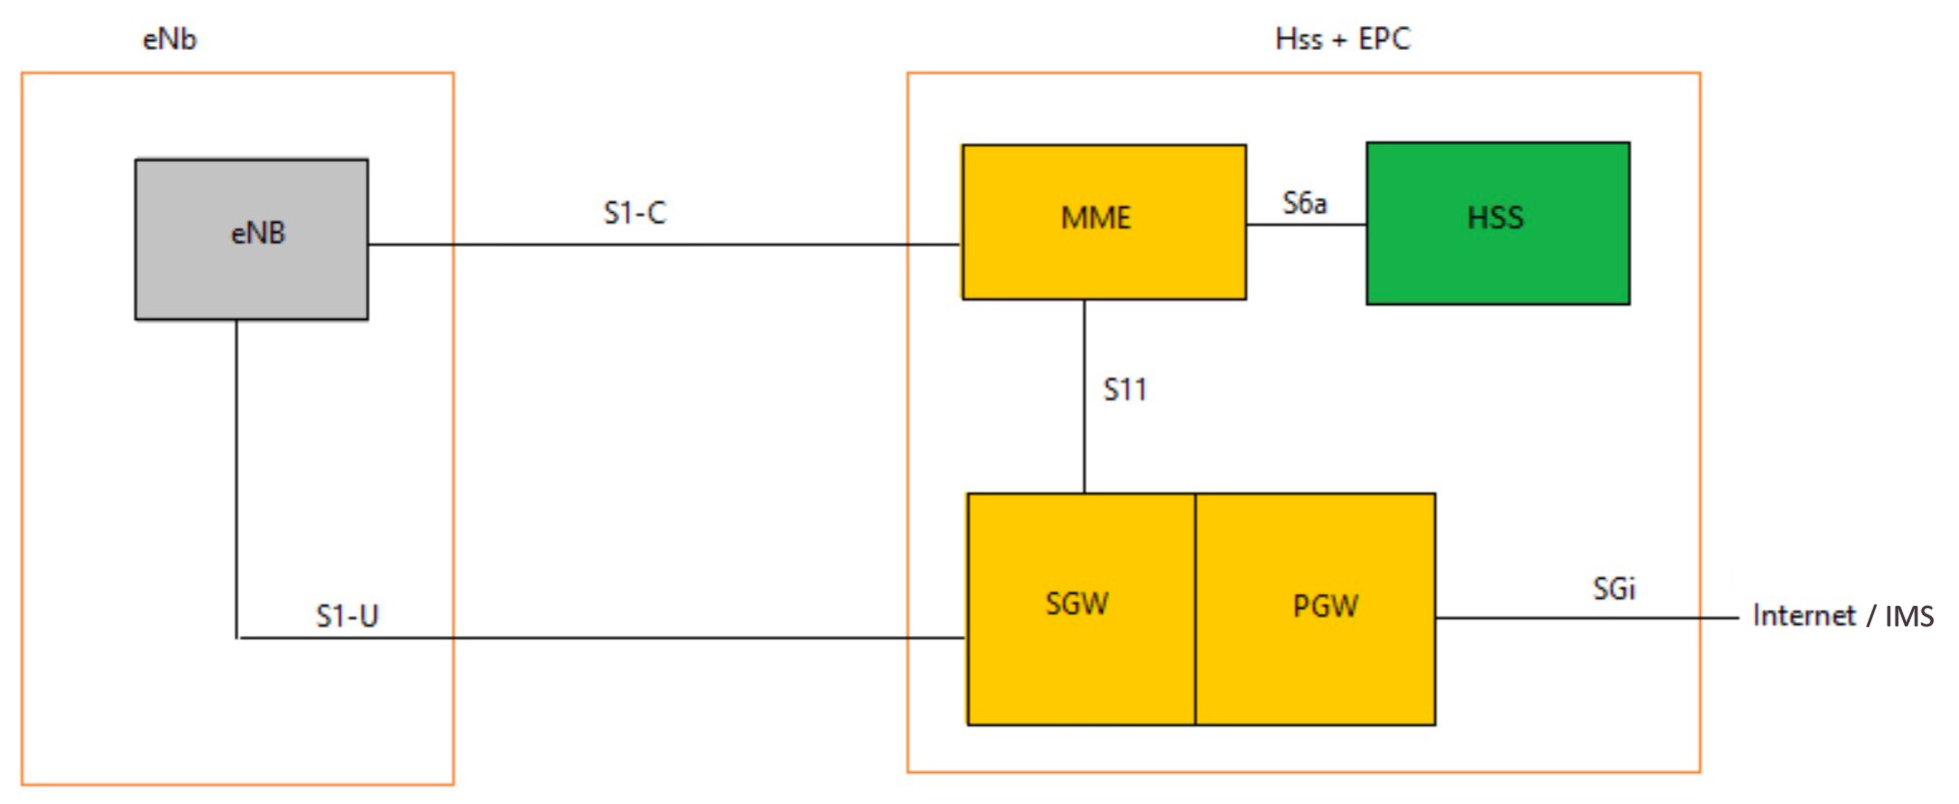
\includegraphics[width=0.75\textwidth]{oai}
\caption{معماری مورد استفاده در پیاده\nf سازی \lr{oai}}
\label{oai}
\end{figure}

در این پروژه، سیستمی که \lr{EPC} و المان \lr{SPGW} روی آن نصب شده است، از طریق شبکه\nf ی داخلی دانشگاه به اینترنت جهانی متّصل می\nf شود. لذا، در پیکربندی \lr{SPGW}، اینترفیس \lr{VPN} به عنوان رابط \lr{SPGW} با شبکه\nf ی خارجی معرّفی شد. در صورت قرار دادن اینترفیس مربوط به شبکه\nf ی داخلی دانشگاه\RTLfootnote{مثلاً می\nf توان اینترفیس وای\nf فای که به یکی از مودم\nf های شبکه\nf ی دانشگاه متّصل است را برای این کار در نظر گرفت. } در پیکربندی مربوطه، می\nf توان ارتباط \lr{oai} با اینترنت جهانی را قطع کرده و صرفاً شبکه\nf ی داخلی دانشگاه را در اختیار مشترکین قرار داد. با این کار، مشترکین قادر به استفاده از شبکه\nf ی دانشگاه و \lr{IMS} خواهندبود ولی دیگر از طریق سیم\nf کارت مربوط به \lr{oai}، نمی\nf توانند به اینترنت جهانی دسترسی داشته\nf باشند. از آنجایی\nf که استفاده از شبکه\nf ی داخلی دانشگاه برای کاربران رایگان است، دیگر لازم نیست که میزان استفاده این کاربران از اینترنت جهانی(از طریق اتّصال دیتای سیم\nf کارت و بدون استفاده از \lr{VPN}) را کنترل کرد. از آنجایی\nf که خدمات شارژینگ در المان \lr{PCRF} انجام می\nf شود و این المان، با عنوان تجاری \lr{Perimeta} به فروش می\nf رسد و ما به آن دسترسی نداریم، این راه\nf حل، کمک به ارائه\nf ی سرویس \lr{IMS} و \lr{LTE} در سطح دانشگاه می\nf کند.


برای اتّصال \lr{IMS} به \lr{oai}، کافی است که دسترسی این دو سیستم به یکدیگر از طریق پروتکل \lr{IP} را فراهم شود. در صورت دسترسی \lr{SPGW} به \lr{IMS} از طریق \lr{IP}، کاربران \lr{oai} نیز قادر به دسترسی به \lr{IMS} هستند و می\nf توانند عملیّات ثبت\nf نام در \lr{IMS} را انجام دهند و تماس تلفنی برقرار کنند. ساده\nf ترین راه برای انجام این کار، اتّصال سیستم \lr{IMS} و \lr{EPC} به یک شبکه\nf ی محلّی مشترک است.

\section{برقراری تماس تلفنی بین کاربران \lr{4G} توسّط \lr{IMS}}

در این پروژه، به\nf منظور برقراری این ارتباط، هر دو سیستم(\lr{EPC} و \lr{IMS}) به مودم وای\nf فای مرکز اوییونیک دانشگاه متّصل شدند. از طریق آدرس \lr{IP} خصوصی که مودم به این دو سیستم اختصاص داد، ارتباط آن\nf ها با یکدیگر برقرار شد و دسترسی دو سیستم به یکدیگر، از طریق \lr{ping} بررسی شد. از پیاده\nf سازی یکپارچه \lr{clearwater} بر روی \lr{Virtulabox} به\nf عنوان سیستم \lr{IMS} استفاده شد. پس از اتّصال تلفن همراه کاربر از طریق سیم\nf کارت به \lr{oai} و روشن کردن دیتای اینترنت تلفن همراه، دسترسی تلفن همراه کاربر به \lr{IMS} فراهم شد. با نصب اپلیکیشن \lr{zoiper} بر روی تلفن همراه و انجام پیکربندی لازم مطابق بخش \ref{zoiperconf}، ثبت\nf نام کاربر در \lr{IMS} با موفقیّت انجام شد. با انجام روشی مشابه، کاربر دوّم نیز به \lr{IMS} متّصل شد. سپس، دو کاربر توانستند با یکدیگر تماس تلفنی برقرار کنند.

\begin{figure}[H]
\centering
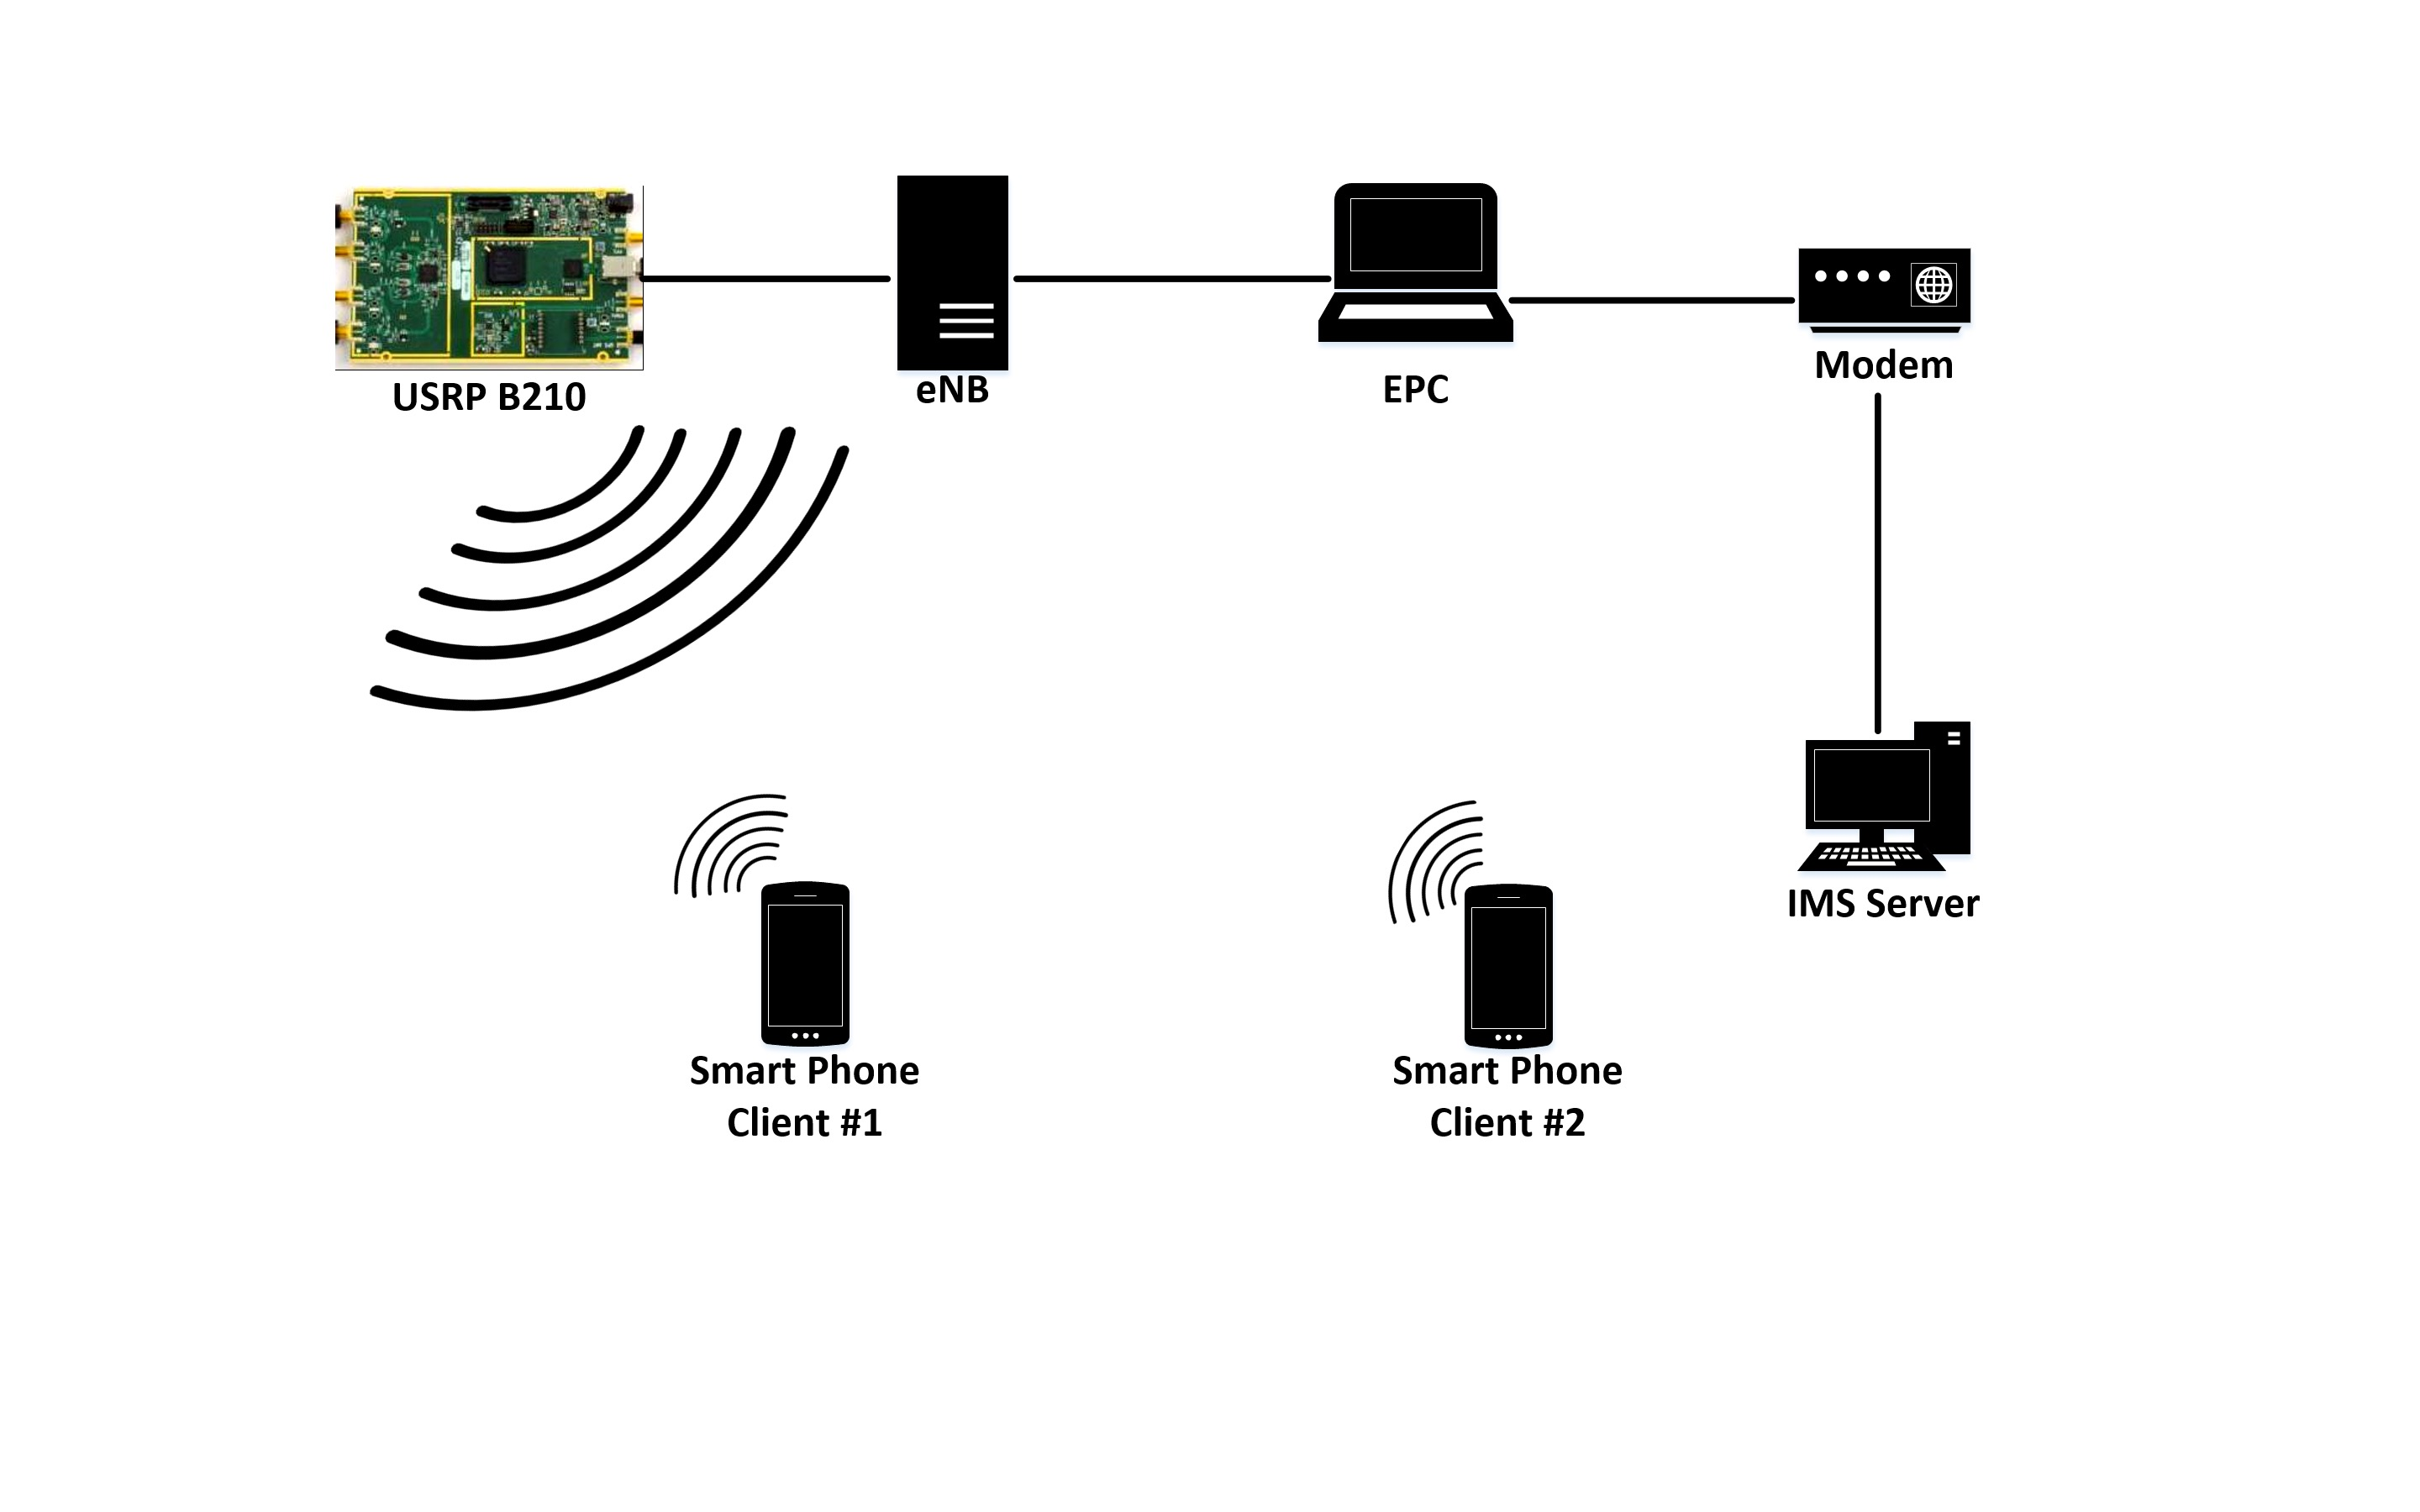
\includegraphics[width=\textwidth]{IMS2VOLTE}
\caption{توپولوژی ارتباط \lr{IMS} و \lr{4G} و برقراری تماس صوتی به\nf وسیله\nf ی این شبکه}
\label{IMS2VOLTE}
\end{figure}